\documentclass[12pt]{article}
\usepackage{amsfonts, amstext, amsmath, amsthm, amscd, amssymb, hyperref, float, longtable, fullpage}
\usepackage{textcomp, gensymb}
\usepackage{epsfig, graphics, psfrag}
\usepackage{graphicx}
\usepackage{subfig}
\graphicspath{{./images/}}
\usepackage{color}
\usepackage[font=small, labelfont=bf]{caption}
\usepackage{float}
\newtheorem{proposition}{Proposition}[section]
\newtheorem{theorem}{Theorem}[section]
\newtheorem{lemma}{Lemma}[section]
\newtheorem{corollary}{Corollary}[section]
\newtheorem{conjecture}{Conjecture}[section]
\newtheorem{claim}{Claim}[section]
\newtheorem{definition}{Definition}[section] 
\let\olddefinition\definition
\renewcommand{\definition}{\olddefinition\normalfont}
\newtheorem{remark}{Remark}[section]
\let\oldremark\remark
\renewcommand{\remark}{\oldremark\normalfont}
\newtheorem{question}{Question}[section]
\let\oldquestion\question
\renewcommand{\question}{\oldquestion\normalfont}
\newtheorem{notation}{Notation}[section]
\let\oldnotation\notation
\renewcommand{\notation}{\oldnotation\normalfont}
\newtheorem{example}{Example}[section]
\let\oldexample\example
\renewcommand{\example}{\oldexample\normalfont}
\newtheorem{algorithm}{Algorithm}[section]
\let\oldalgortihm\algorithm
\renewcommand{\algorithm}{\oldalgorithm\normalfont}
\newtheorem{method}{Method}[section]
\let\oldmethod\method
\renewcommand{\method}{\oldmethod\normalfont}
\let\oldemptyset\emptyset
\let\emptyset\varnothing
\newcommand{\ndiv}{\hspace{-4pt}\not|\hspace{2pt}}
\newcommand{\vect}[1]{\boldsymbol{#1}}

\setlength{\parindent}{0in}
\setcounter{MaxMatrixCols}{20}

%%%%%%%%%%%%%%%%%%%%%%%%%%%%%%%%%%%%%%%%%%%%%%%%%%%%%%%%%%%%%%%%%%%%%%%%%%%%%%%%%%%%%%%%%%%%%%%%%%%%%%%%%%%%%%%%%%%%%%%



\title{{\bf{ECE 3111}} \\ Design and Simulation of a Quadcopter using Simulink}

\author{Alexander Gmuer}

\date{\today}

%%%%%%%%%%%%%%%%%%%%%%%%%%%%%%%%%%%%%%%%%%%%%%%%%%%%%%%%

\begin{document}

\maketitle

\section*{Introduction}

The quadcopter is one of the more well known and useful aerial drones, and its use only continues 
to rise. Instrumental to this has been computer simulation tools, like MATLAB and Simulink, which improve the 
efficiency and design of the quadcopter as a control system. The goal of this paper is to document the development 
of a quadcopter system from first principles, and then demonstrate the system response when the quadcopter takes off from
the ground and stabilizes at a height of 5 meters.  

\begin{figure}[h]
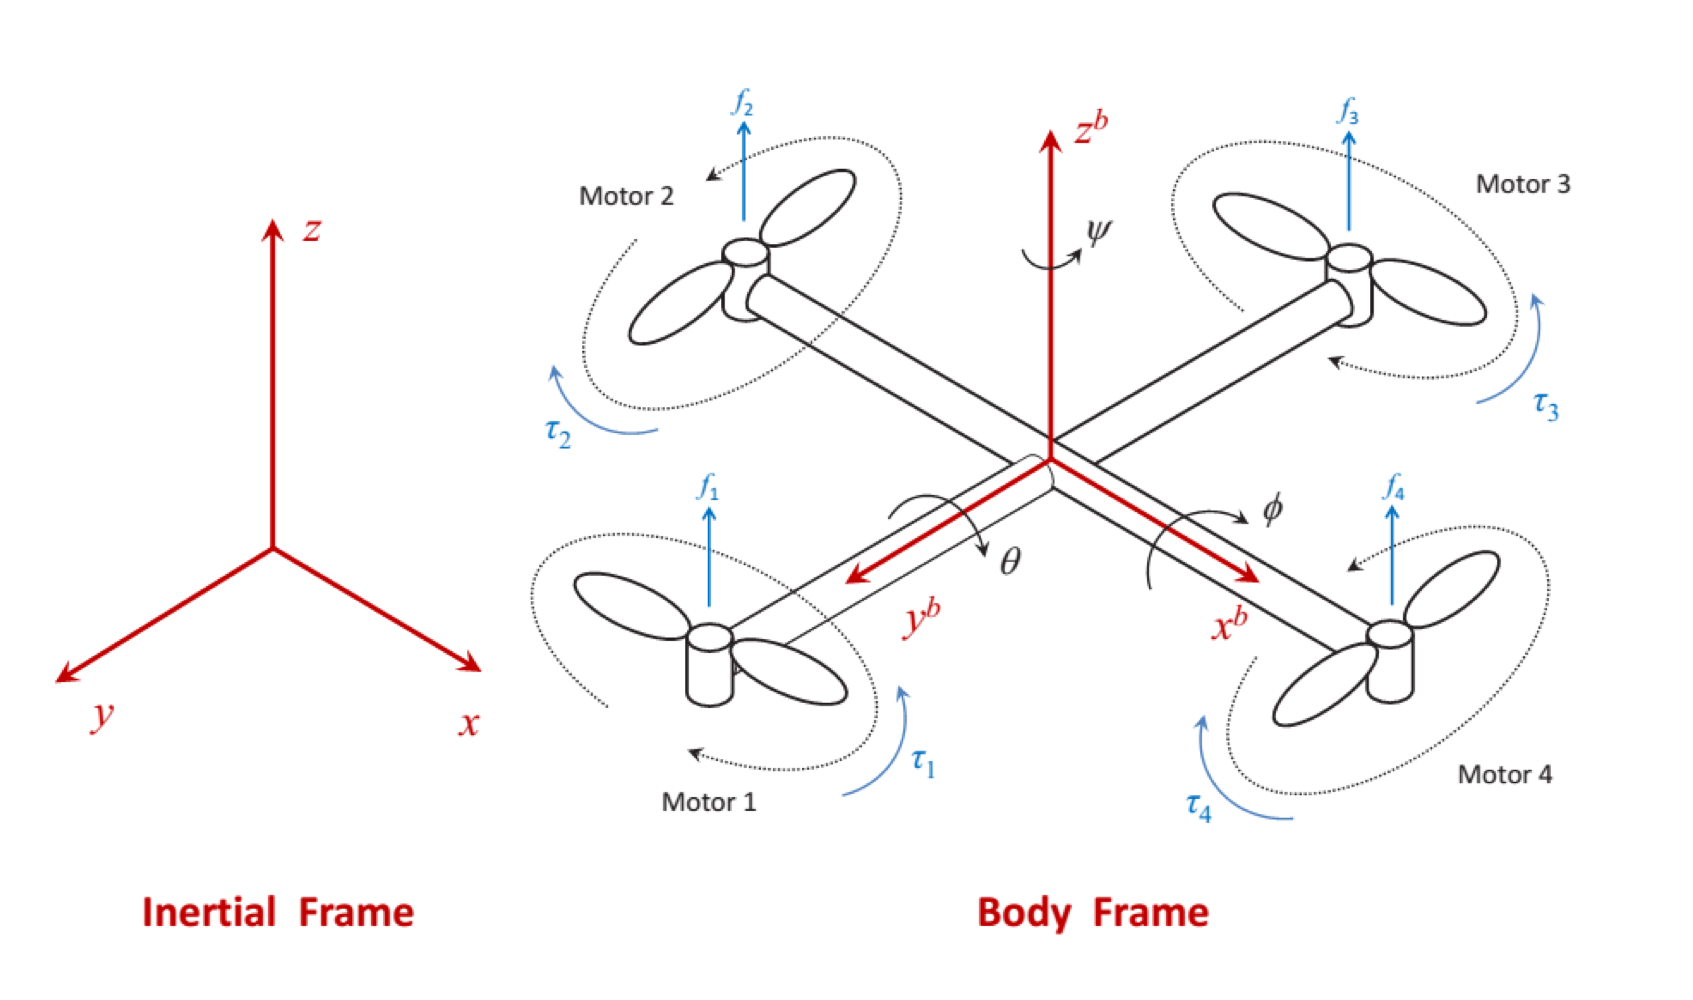
\includegraphics[scale=0.2]{images/Quadcopter Inertial Frame.png}
\centering
\end{figure}

\section{Linearization}

Given the diagram shown above of the quadcopter in space, non-linear equations of motion can be derived
which describe the mechanics of the system. These equations relate the square voltage motor inputs $u_1,u_2,u_3,$ and $u_4$ to
the positions, velocities, and accelerations in the $x,y,$ and $z$ directions - as well as the pitch ($\phi$), roll ($\theta$), 
and yaw ($\psi$) of the quadcopter with respect to its inertial reference frame:
\begin{align*}
    \dot{x} &= v_x \\
    \dot{y} &= v_y \\
    \dot{z} &= v_z \\
    \dot{v_x} &= -\frac{k_d}{m}v_x + \frac{kc_m}{m}(\sin\psi\sin\phi + \cos\psi\cos\phi\sin\theta)(u_1 + u_2 + u_3 + u_4) \\
    \dot{v_y} &= -\frac{k_d}{m}v_y + \frac{kc_m}{m}(\cos\phi\sin\psi\sin\theta - \cos\psi\sin\phi)(u_1 + u_2 + u_3 + u_4)\\
    \dot{v_z} &= -\frac{k_d}{m}v_z -g + \frac{kc_m}{m}(\cos\theta\cos\phi)(u_1 + u_2 + u_3 + u_4) \\
    \dot{\phi} &= \omega_x + \omega_y(\sin\phi\tan\theta) + \omega_z(\cos\phi\tan\theta) \\
    \dot{\theta} &= \omega_y(\cos\phi) + \omega_z(-\sin\theta) \\
    \dot{\psi} &= \omega_y(\sin\phi/\cos\theta) + \omega_z(\cos\phi/\cos\theta) \\
    \dot{\omega_x} &= \frac{Lkc_m}{I_{xx}}(u_1 - u_3) - \left((\frac{I_{yy} - I_{zz}}{I_{xx}}\right)\omega_y \omega_z \\
    \dot{\omega_y} &= \frac{Lkc_m}{I_{yy}}(u_2 - u_4) - \left(\frac{I_{zz} - I_{xx}}{I_{yy}}\right)\omega_x \omega_z \\
    \dot{\omega_z} &= \frac{Lkc_m}{I_{zz}}(u_1 - u_2 + u_3 - u_4) - \left(\frac{I_{xx} - I_{yy}}{I_{zz}}\right)\omega_x \omega_y \\
\end{align*}

In order to create a robust model which is able to be analyzed by typical control methods, 
the equations of motion above must be linearized. We shall consider the 
system equilibrium point at which $x = y = z = 0m$, and $\phi = \theta = \psi = 0^{\circ}$.
The equations of motion can then be put in a linear form:
\begin{equation}
  \begin{split}
    \dot{x} &= v_x \\
    \dot{y} &= v_y \\
    \dot{z} &= v_z \\
    \dot{v_x} &= -\frac{k_d}{m}v_x +  \\
    \dot{v_y} &= -\frac{k_d}{m}v_y + \\
    \dot{v_z} &= -\frac{k_d}{m}v_z -g + \frac{kc_m}{m}(u_1 + u_2 + u_3 + u_4) \\
  \end{split}
\quad\quad
  \begin{split}
    \dot{\phi} &= \omega_x  \\
    \dot{\theta} &= \omega_y \\
    \dot{\psi} &= \omega_z(\cos\phi/\cos\theta) \\
    \dot{\omega_x} &= \frac{Lkc_m}{I_{xx}}(u_1 - u_3) \\
    \dot{\omega_y} &= \frac{Lkc_m}{I_{yy}}(u_2 - u_4)  \\
    \dot{\omega_z} &= \frac{Lkc_m}{I_{zz}}(u_1 - u_2 + u_3 - u_4) \\
  \end{split}
\end{equation}

Having now created a list of approximate linear equations which describe the 
quadcopter system near equilibrium, it can now be modeled as a Multi-Input, Multi-Output
(MIMO) system using state space representation in the time domain. 

\section{Modeling the System: State Space \& Transfer Function}

Before constructing the state space quadcopter model, it is important to remind ourselves 
of the desired inputs and outputs for this system. This is a matter of design and perspective,
as most modern systems are complex and layered, with engineering teams often only responsible
for a single subsystem. In the case of the quadcopter, our model is designed to take squared
voltages for each of the four motors as inputs, then use those to control the attitude, 
(roll, pitch, and yaw) as well as the altitude and and position. 
\par
Looking at the linearized equations of motion, we see that $u_1, u_2, u_3,$ and $u_4$ are the 
input motor voltages, and the outputs are $x,y,z,\phi,\theta,$ and $\psi$. This means that this 
system will have 4 inputs and 6 outputs. In the state space model, this means that the input $\textbf{u}$
vector will contain the squared motor voltages $u_1, u_2, u_3,$ and $u_4$. The output $\textbf{y}$ vector, 
meanwhile, will contain the $x,y,z,\phi,\theta,$ and $\psi$ state variables. With this, as well as the 
linearized equations of motion, we can construct the state space representation:
\begin{align*}
  \dot{\textbf{x}} &= A\textbf{x} + B\textbf{u} \\
  \textbf{y} &= C\textbf{x} + D\textbf{u} 
\end{align*}
Where the matrices $A$ and $B$ are given by:
\begin{equation*}
  \begin{split}
  A &= 
  \begin{bmatrix}
  0 & 0 & 0 & 1 & 0 & 0 & 0 & 0 & 0 & 0 & 0 & 0 \\
  0 & 0 & 0 & 0 & 1 & 0 & 0 & 0 & 0 & 0 & 0 & 0 \\
  0 & 0 & 0 & 0 & 0 & 1 & 0 & 0 & 0 & 0 & 0 & 0 \\
  0 & 0 & 0 & \frac{-kd}{m} & 0 & 0 & 0 & 0 & 0 & 0 & 0 & 0 \\
  0 & 0 & 0 & 0 & \frac{-kd}{m} & 0 & 0 & 0 & 0 & 0 & 0 & 0 \\
  0 & 0 & 0 & 0 & 0 & \frac{-kd}{m} & 0 & 0 & 0 & 0 & 0 & 0 \\
  0 & 0 & 0 & 0 & 0 & 0 & 0 & 0 & 0 & 1 & 0 & 0 \\
  0 & 0 & 0 & 0 & 0 & 0 & 0 & 0 & 0 & 0 & 1 & 0 \\
  0 & 0 & 0 & 0 & 0 & 0 & 0 & 0 & 0 & 0 & 0 & 1 \\
  0 & 0 & 0 & 0 & 0 & 0 & 0 & 0 & 0 & 0 & 0 & 0 \\
  0 & 0 & 0 & 0 & 0 & 0 & 0 & 0 & 0 & 0 & 0 & 0 \\
  0 & 0 & 0 & 0 & 0 & 0 & 0 & 0 & 0 & 0 & 0 & 0 
  \end{bmatrix} \\
  \end{split}
\quad\quad
  \begin{split}
  B &= 
  \begin{bmatrix}
  0 & 0 & 0 & 0  \\
  0 & 0 & 0 & 0  \\
  0 & 0 & 0 & 0  \\
  0 & 0 & 0 & 0 \\
  0 & 0 & 0 & 0 \\
  \frac{kc_m}{m} & \frac{kc_m}{m} & \frac{kc_m}{m} & \frac{kc_m}{m} \\
  0 & 0 & 0 & 0 \\
  0 & 0 & 0 & 0 \\
  0 & 0 & 0 & 0 \\
  \frac{Lkc_m}{I_{xx}} & 0 & -\frac{Lkc_m}{I_{xx}} & 0 \\
  0 & \frac{Lkc_m}{I_{yy}} & 0 & -\frac{Lkc_m}{I_{yy}} \\
  \frac{Lbc_m}{I_{zz}} & -\frac{Lbc_m}{I_{zz}} & \frac{Lbc_m}{I_{zz}} & -\frac{Lbc_m}{I_{zz}} 
  \end{bmatrix} \\
  \end{split}
\end{equation*}
While the $D$ matrix is zero, and $C$ is given by:
\begin{align*}
  C &= 
  \begin{bmatrix}
  1 & 0 & 0 & 0 & 0 & 0 & 0 & 0 & 0 & 0 & 0 & 0 \\
  0 & 1 & 0 & 0 & 0 & 0 & 0 & 0 & 0 & 0 & 0 & 0 \\
  0 & 0 & 1 & 0 & 0 & 0 & 0 & 0 & 0 & 0 & 0 & 0 \\
  0 & 0 & 0 & 0 & 0 & 0 & 1 & 0 & 0 & 0 & 0 & 0 \\
  0 & 0 & 0 & 0 & 0 & 0 & 0 & 1 & 0 & 0 & 0 & 0 \\
  0 & 0 & 0 & 0 & 0 & 0 & 0 & 0 & 1 & 0 & 0 & 0 \\
  \end{bmatrix} \\
\end{align*}
The matrix dimensions of $A, B,$ and $C$ are thus:
\begin{align*}
  A &: 12\times12\\
  B &: 12\times4\\
  C &: 6\times12\\
\end{align*}
Using the matrix equation $T_{ij}(s) = C_i(sI - A)^{-1}B_j + D$, 
a $6\times4$ transfer function matrix $T$ can be calculated, such that:
  $$\textbf{y} = T\textbf{u}$$
Where we have $T$ to be:
\begin{align*}
  T &= 
  \begin{bmatrix}
    0 & 0 & 0 & 0 \\
    0 & 0 & 0 & 0 \\[6pt]
    \frac{3}{25s(2s + 1)} & \frac{3}{25s(2s + 1)} & \frac{3}{25s(2s + 1)} & \frac{3}{25s(2s + 1)} \\[6pt]
    \frac{3}{2s^2} & 0 & -\frac{3}{2s^2} & 0 \\[6pt]
    0 & \frac{3}{2s^2} & 0 & -\frac{3}{2s^2} \\[6pt]
    \frac{1}{40s^2} & -\frac{1}{40s^2} & \frac{1}{40s^2} & -\frac{1}{40s^2} \\[6pt]
  \end{bmatrix}
\end{align*}
Since the first two rows of the transfer function matrix are zero, and correspond to the $x$ and $y$ responses,
for the remainder of the model we will consider $T$ as a $4\times4$ matrix composing of the transfer functions
for the $z,\phi, \theta,$ and $\psi$ variables.
\section{Control Conversion}

Using the relation $\omega_i = c_mu_i$ for $i = 1,2,3,4$, 
which relates the input squared voltages $u_i$ to the squared angular velocities of the corresponding motors.
The angular velocities of the motors can be further related to the $z,\phi, \theta,$ and $\psi$ inputs via 
the following mapping:
\begin{align*}
  \begin{bmatrix}
    u_z \\
    u_{\phi} \\
    u_{\theta} \\
    u_{\psi} 
  \end{bmatrix}
  &= 
  \begin{bmatrix}
    0.5 & 0.5 & 0.5 & 0.5 \\
    0.5 & -0.5 & 0 & 0 \\
    1 & 0 & -0.5 & -0.5 \\
    0 & 0 & 0.5 & -0.5 \\
  \end{bmatrix}
  \begin{bmatrix}
    \omega_1^2 \\
    \omega_2^2 \\
    \omega_3^2 \\
    \omega_4^2 \\
  \end{bmatrix}
\end{align*}
Using this mapping matrix $M$, the transfer function matrix $T$ can be converted
so that it can take inputs $u_z, u_{\phi}, u_{\theta},$ and $u_{\psi}$
through the following steps:
\begin{align*}
   \textbf{y} &= T*\textbf{u} \\
   \textbf{u'} &= M*c_m*\textbf{u} \\
   \implies \textbf{u} &= M^{-1}*\frac{1}{c_m}*\textbf{u'} \\
   \implies \textbf{y} &= T*M^{-1}*\frac{1}{c_m}*\textbf{u'} \\
\end{align*}
Where $\textbf{u'} = [u_z \ u_{\phi} \ u_{\theta} \ u_{\psi}]^T$. This transformation results in 
the following transfer function matrix:
\[
  H =
\begin{bmatrix}
  \frac{3}{125000s(2s + 1)} & 0 & 0 & 0 \\[6pt]
    0 & -\frac{3}{20000s^2} & -\frac{3}{20000s^2} & 0 \\[6pt]
    0 & \frac{3}{20000s^2} & \frac{3}{20000s^2} & -\frac{3}{10000s^2} \\[6pt]
    0 &  \frac{1}{20000s^2}&  & \frac{1}{20000s^2} \\[6pt]
\end{bmatrix}
\]
Taking the transfer functions along the diagonal entries, we can attain a set of open loop transfer functions
which can model the four control variables:
\begin{align*}
  \frac{Z(s)}{U_z(s)} &= \frac{3}{125000s(2s + 1)}\\
  \frac{\phi(s)}{U_{\phi}(s)} &= -\frac{3}{20000s^2}\\
  \frac{\theta(s)}{U_{\theta}(s)} &= \frac{3}{20000s^2}\\
  \frac{\psi(s)}{U_{\psi}(s)} &= \frac{1}{20000s^2}
\end{align*} 
\section{PID Control Design \& Analysis}
The next step of the system design was to determine how P, PI, and PID controllers influenced
the stability of the system. Luckily, since all of the above four transfer functions have either 
one or two poles at the origin, they are each either Type 1 or Type 2 systems - which means that
in the absence of any proportional gain, the system as a whole is only marginally stable in response
to a standard step input. By adding a proportional gain or P controller, the system would be stable 
for the $z$ translation, but it will still be marginally stable in terms of the attitude angles. Therefore
a P controller would be sufficient to stabilize the $Z$ translation subsystem, however a PI controller will
be necessary for stability for attitudinal stability of the quadcopter.
\par
Despite the fact that a P and PI controller are all that is necessary for stability in our system, 
I opted to design the system with a PID controller in order to control the transient response more 
precisely, as well as to eliminate steady state error in the system response. Adding an integrating I term
to the system allows for the system to handle steady state error, while adding the derivative D term
allows the ability of controlling the settling time, as well as percent overshoot of the system. In short, 
utilizing a PID controller is good for systems which have specific parameter and transient response requirements.
\par
The block diagram of the system, with PID controllers added for each of the four transfer functions, can be seen below:
\begin{figure}[h]
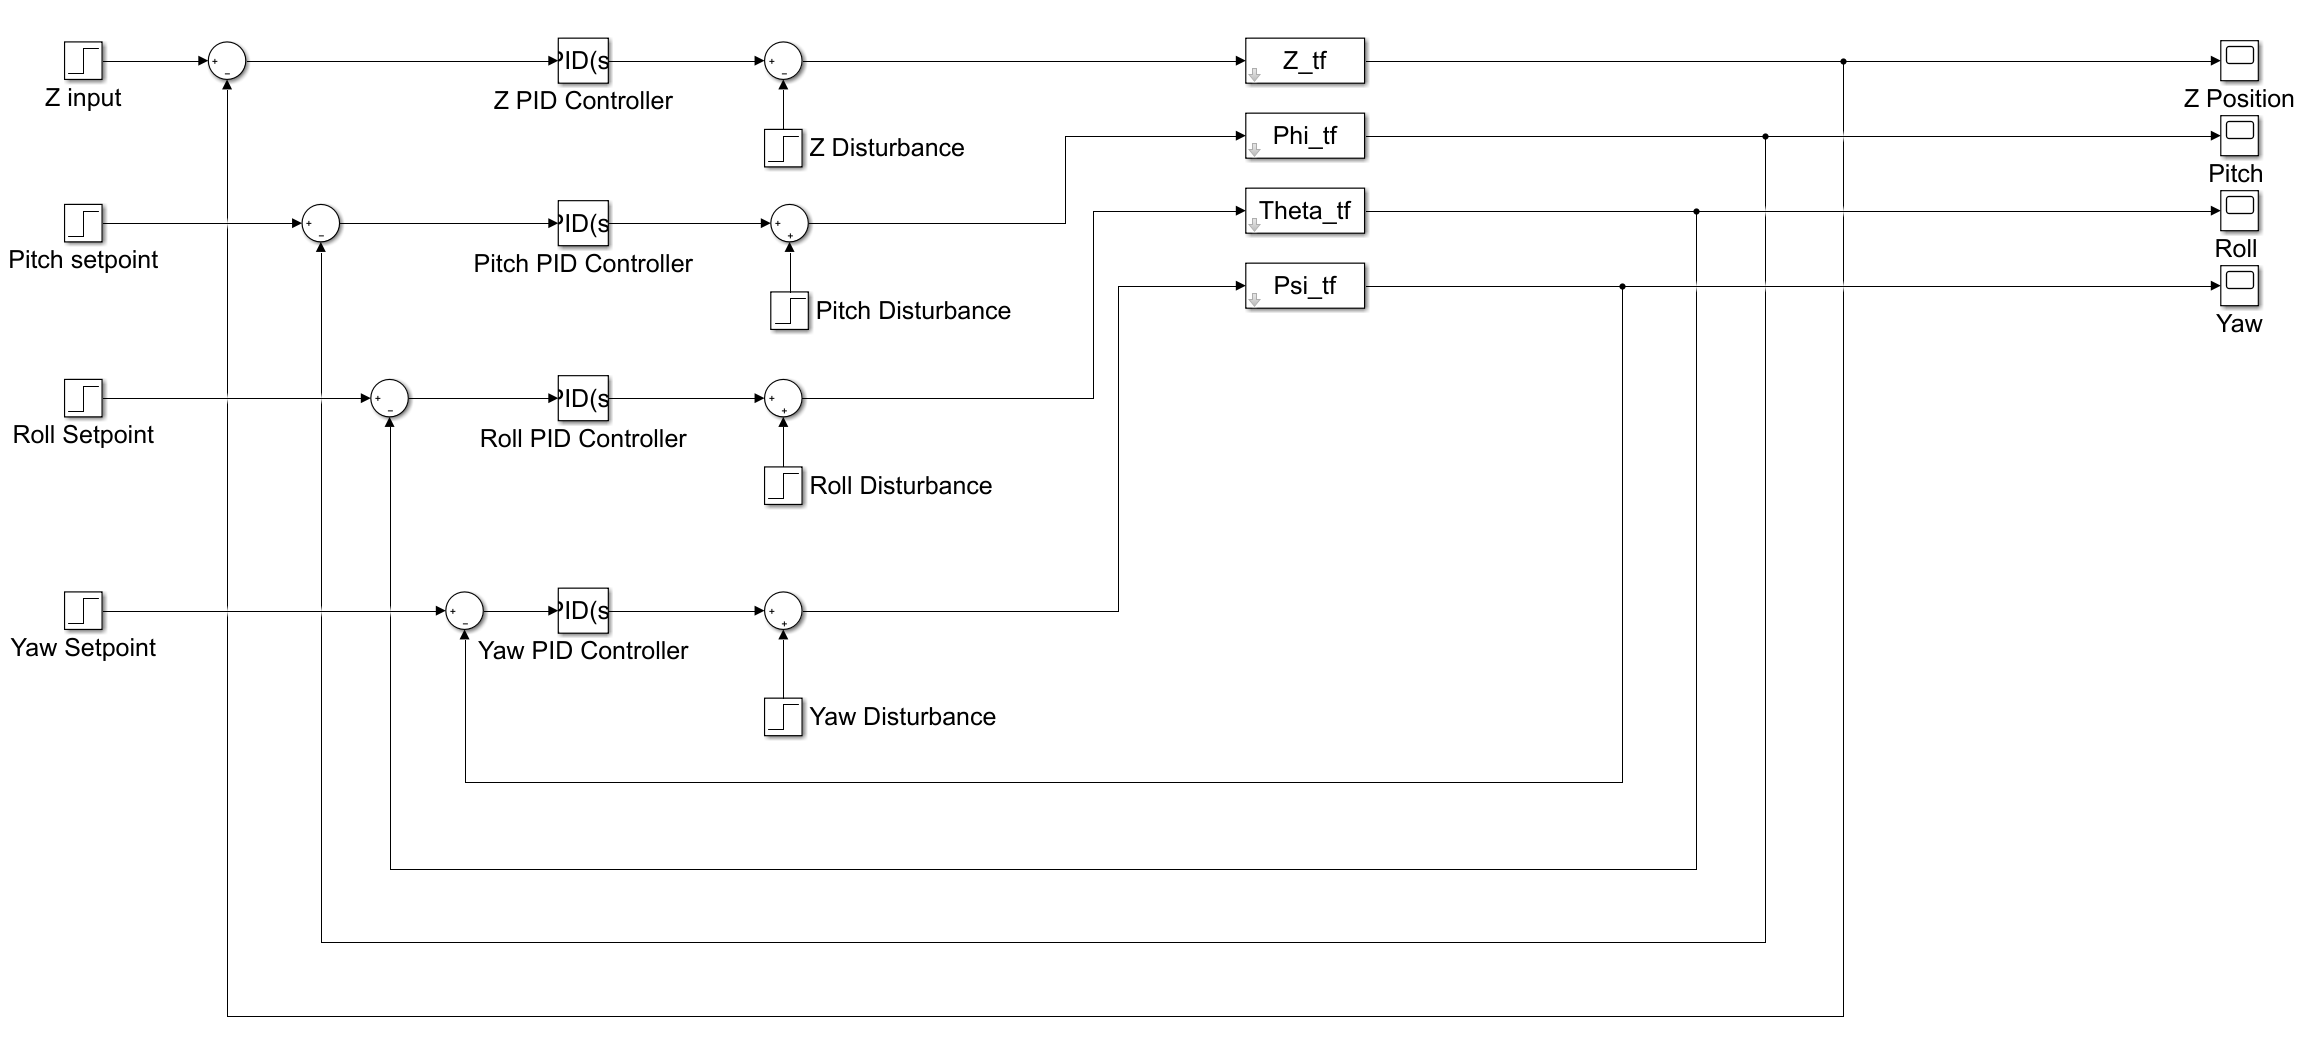
\includegraphics[width=\linewidth]{images/system_block_diagram.png}
\centering
\end{figure}
\subsection*{PID Design}
The table below displays the gain factors associated with the PID controllers in for the $Z$ translation, Pitch, Roll, and Yaw subsystems:
\begin{center}
  \begin{tabular}{||c c c c c||} 
  \hline
   & $Z$ Translation & Pitch & Roll & Yaw \\ [0.5ex] 
  \hline\hline
  $K_p$ & 117450 & -19618 & 21511 & 707609 \\ 
  \hline
  $K_i$ & 21317 & -3656 & 4198 & 144602 \\
  \hline
  $K_d$ & 161472 & -25848 & 27066 & 850263 \\
  \hline
 \end{tabular}
\end{center}
Using these gain values, the system responses were graphed versus time. In the case of the $Z$ translation, the system was provided a 
step input of magnitude 5m, which allows us to see the system response starting at ground level (0 meters) and rising then stabilizing at 5 meters.
The pitch, roll, and roll responses were given as inputs the desired $0^{\circ}$ angles, then given a disturbance step input.
\begin{figure}[h]
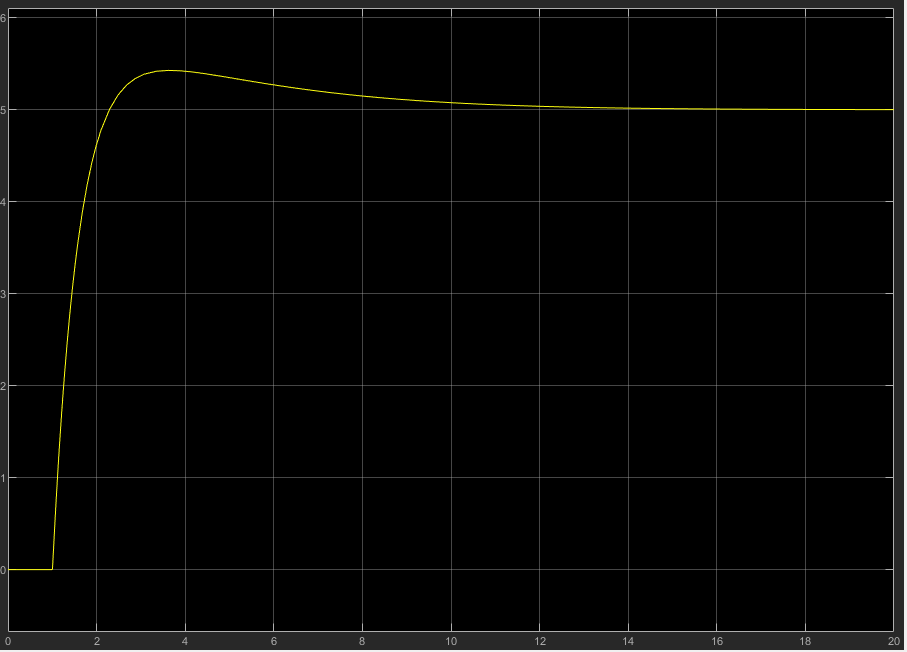
\includegraphics[width=0.9\linewidth]{images/Z_response.png}
\centering
\end{figure}

\begin{figure}[h]
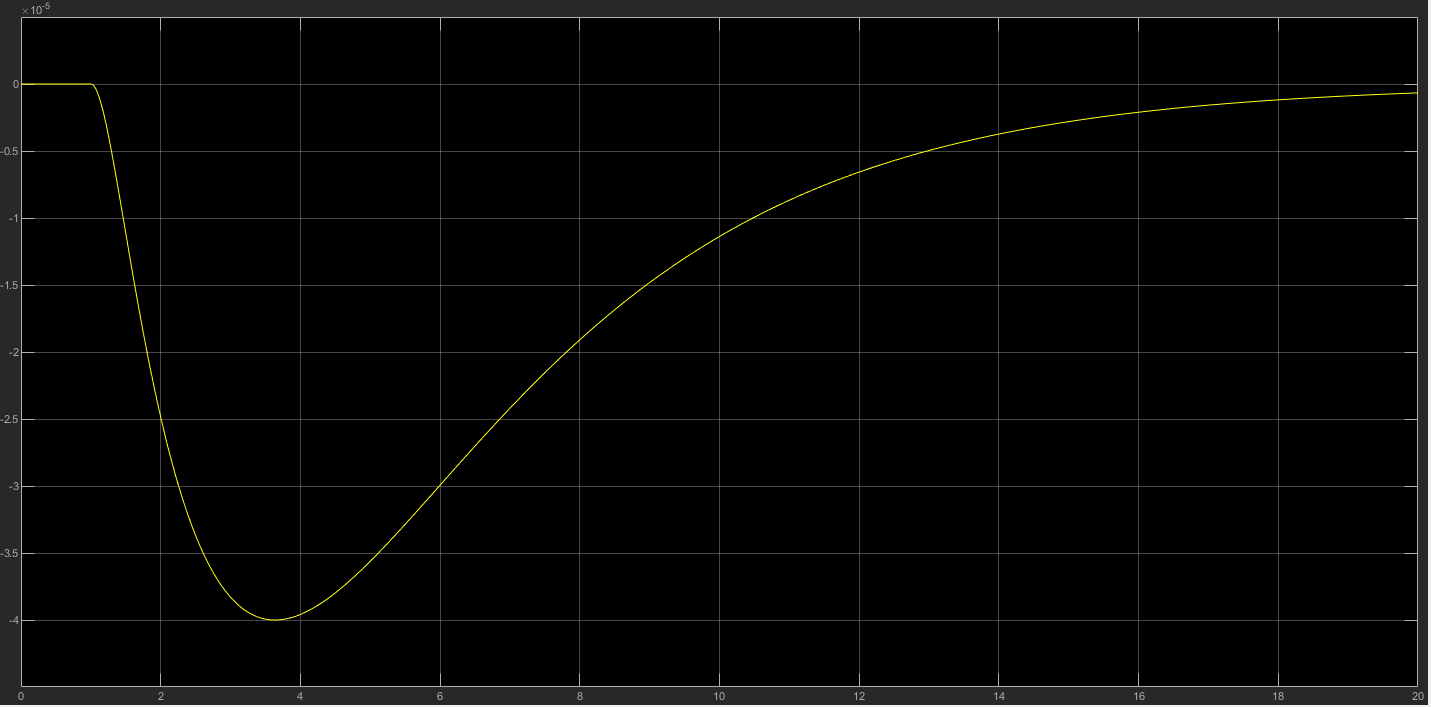
\includegraphics[width=0.9\linewidth]{images/Pitch_response.png}
\centering
\end{figure}

\begin{figure}[h]
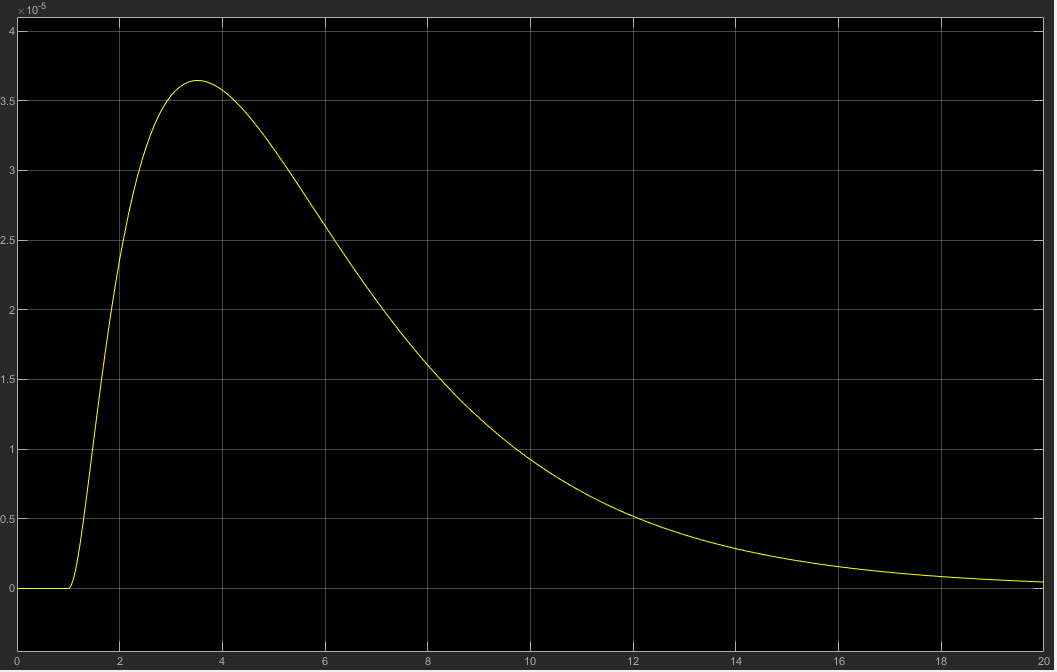
\includegraphics[width=0.9\linewidth]{images/Roll_response.png}
\centering
\end{figure}

\begin{figure}[h]
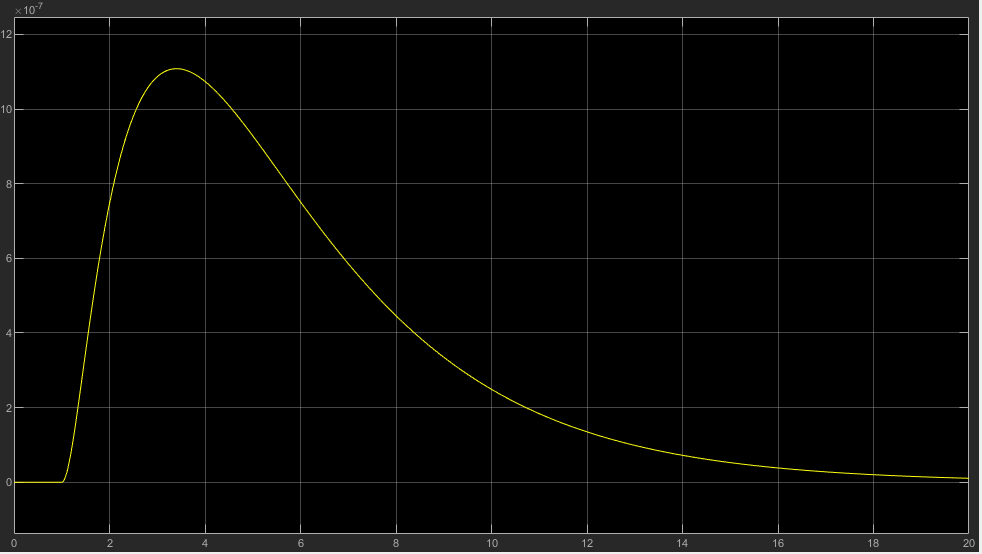
\includegraphics[width=0.9\linewidth]{images/Yaw_response.png}
\centering
\end{figure}

\begin{figure}[h]
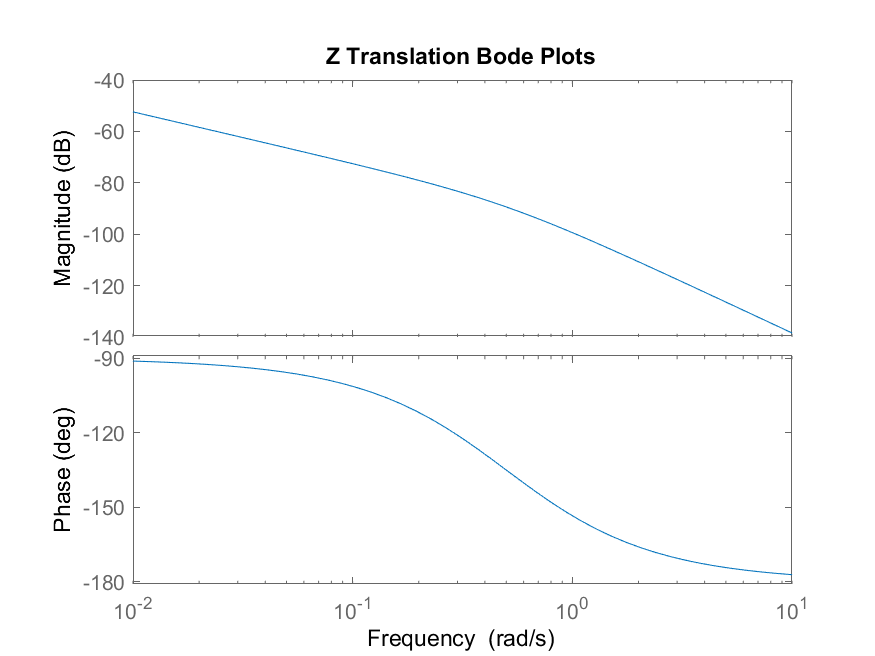
\includegraphics[width=0.75\linewidth]{images/Z_bode.png}
\centering
\end{figure}

\begin{figure}[h]
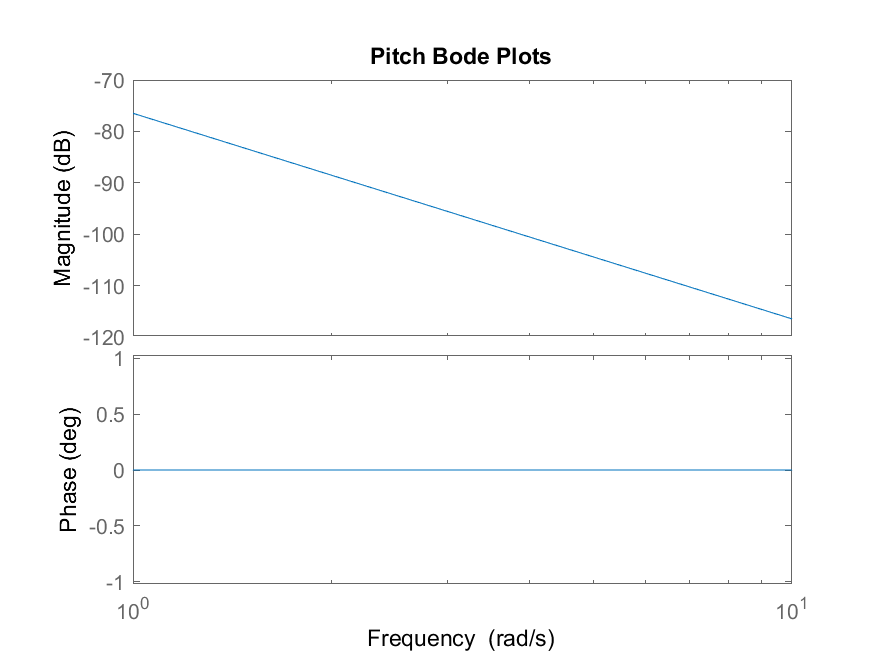
\includegraphics[width=0.75\linewidth]{images/Pitch_bode.png}
\centering
\end{figure}

\begin{figure}[h]
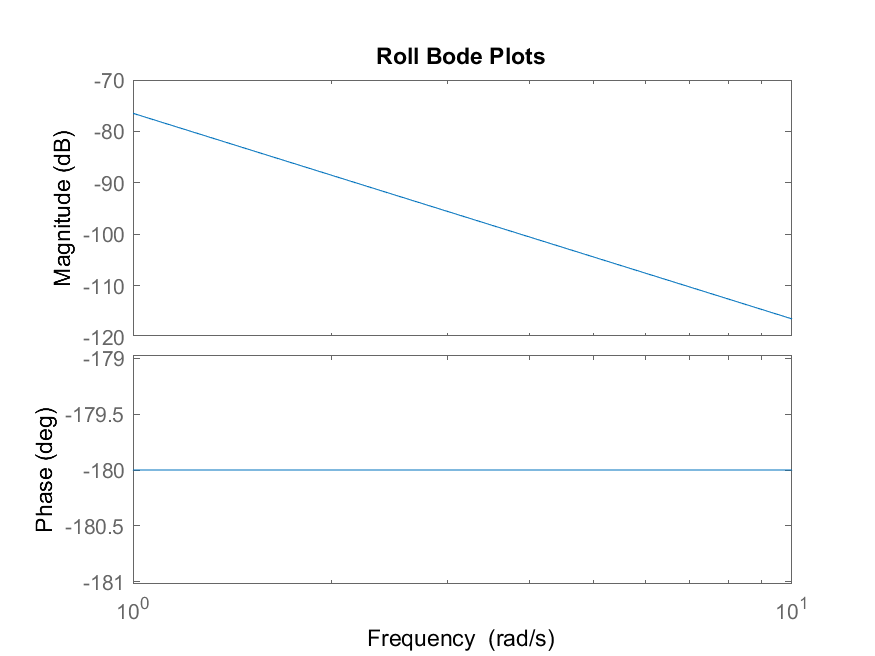
\includegraphics[width=0.75\linewidth]{images/Roll_bode.png}
\centering
\end{figure}

\begin{figure}[h]
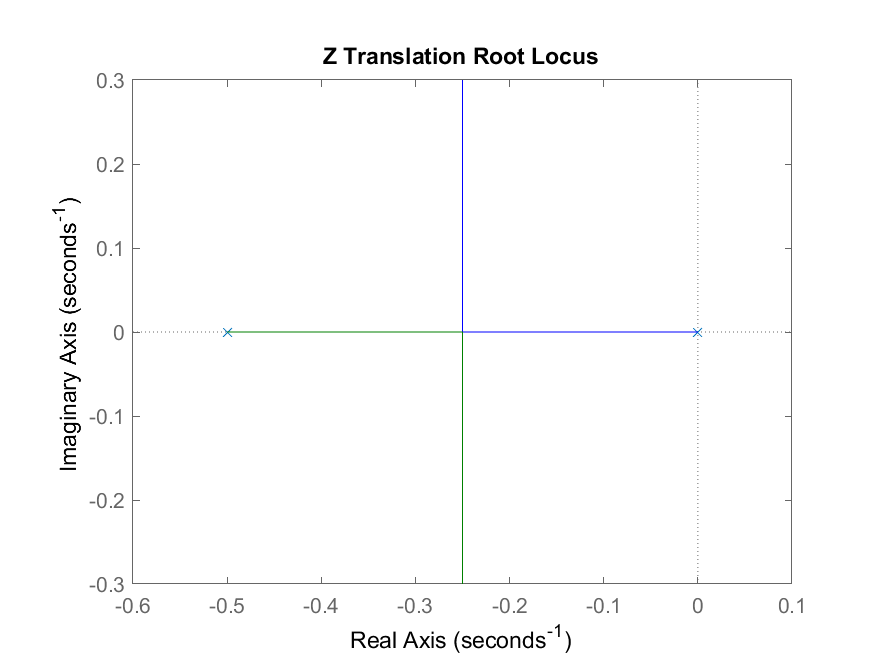
\includegraphics[width=0.75\linewidth]{images/Z_rootlocus.png}
\centering
\end{figure}

\begin{figure}[h]
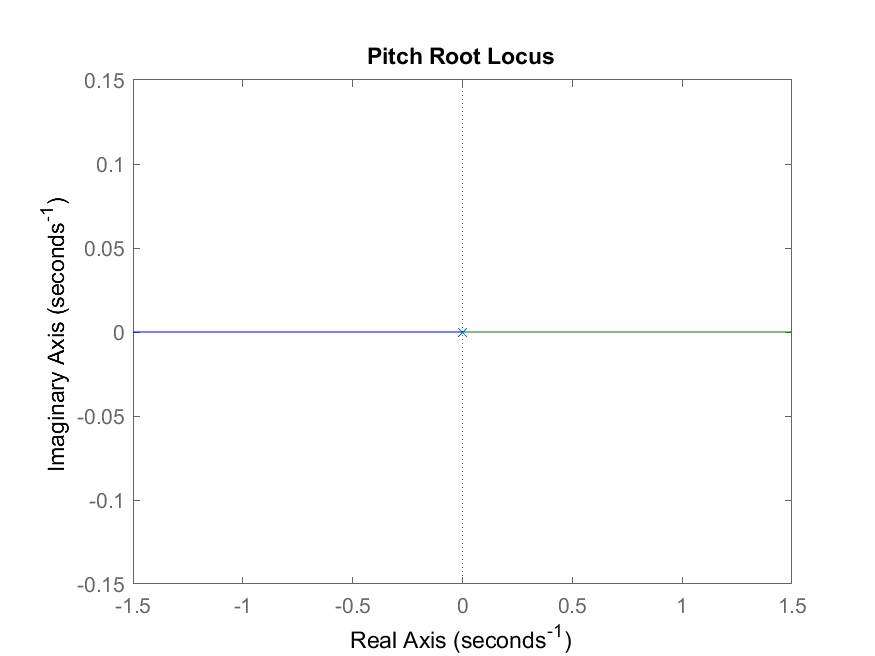
\includegraphics[width=0.75\linewidth]{images/Pitch_rootlocus.png}
\centering
\end{figure}

\begin{figure}[h]
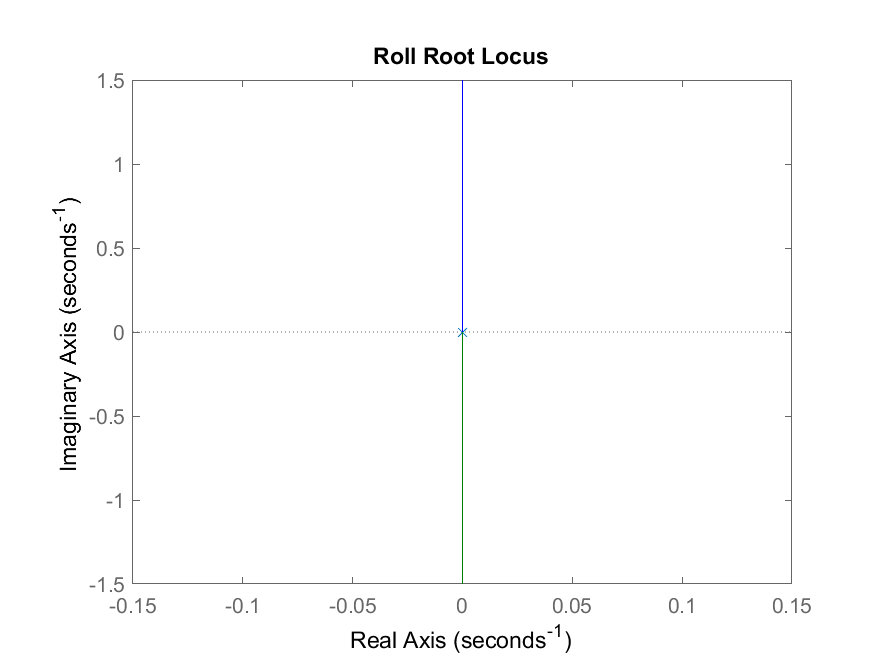
\includegraphics[width=0.75\linewidth]{images/Roll_rootlocus.png}
\centering
\end{figure}

\begin{figure}[h]
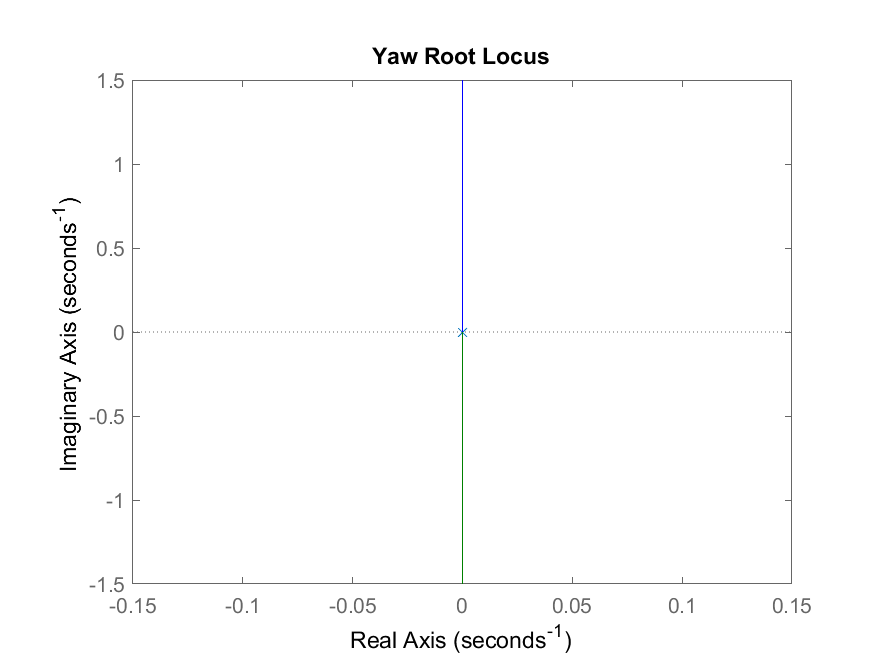
\includegraphics[width=0.75\linewidth]{images/Yaw_rootlocus.png}
\centering
\end{figure}


\end{document}